% XXX Jedes Jahr Professoren-Texte aktualisieren!
\section{Eure Professoren stellen sich vor}
\textbf{Auf den folgenden zwei Seiten stellen sich eure beiden Physik-Professoren vor.
	Sie werden gemeinsam die "Physik~I" bis "Physik~III" lesen.
	Prof.\ Krüger wird sich dabei um die theoretischen und Prof.\ Kappes um die experimentellen Aspekte des Studiums kümmern.
	Zudem stellt sich Prof.\ Werner vor, der die Vorlesungen "Mathematik für Physiker" halten wird (ebenfalls über drei Semester).
	Da diese drei Professoren euch eine Zeit lang begleiten werden, ist es durchaus mal interessant zu wissen, was sie gemacht haben, bevor sie an die Uni Münster kamen, und wie ihre aktuelle Forschung aussieht.}

\begin{multicols}{2}
\begin{center}
	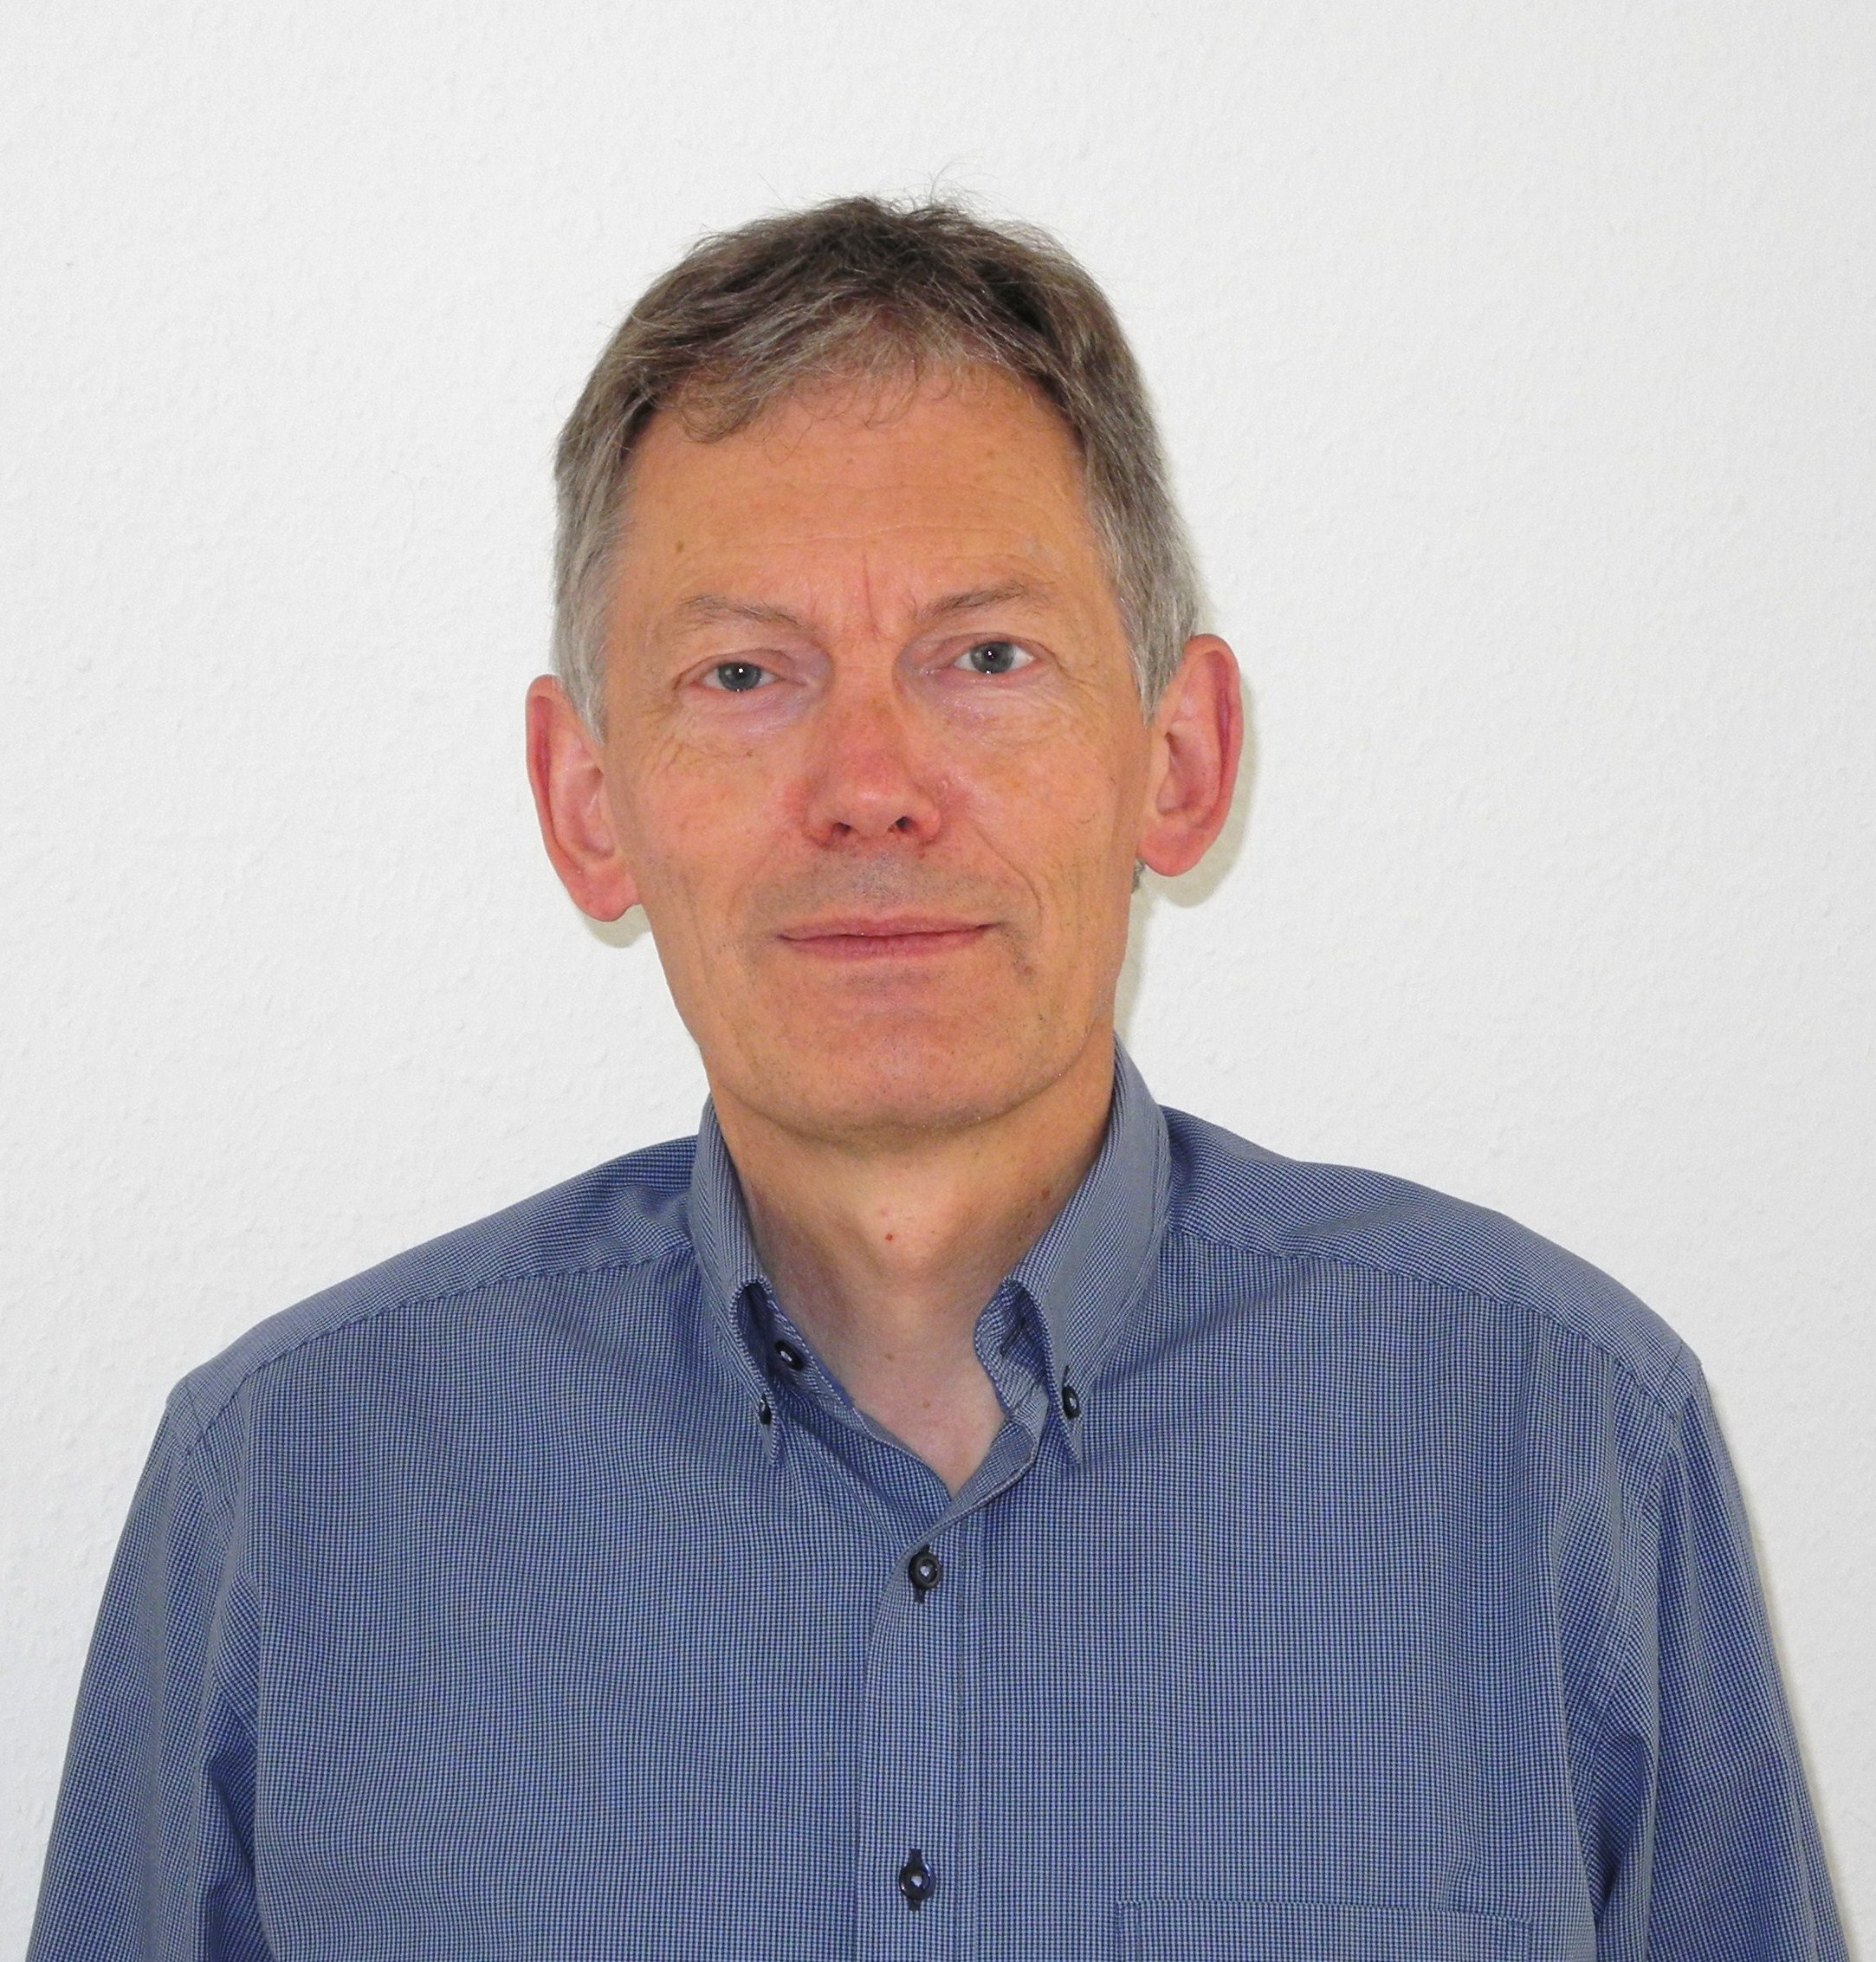
\includegraphics[width=\columnwidth, height=0.35\textheight]{res/vorstellungsfotos/peter_krueger_cropped.jpg}\\
	Apl.\ Prof.\ Dr.\ Peter Krüger\\
	Institut für Festkörpertheorie
\end{center}

In der ersten Hälfte Ihres Physik-Bachelorstudiums werde ich Sie als "Theoretiker" durch den integrierten Kurs Physik~1--3 begleiten und, zusammen mit Prof.\ Dr.\ A.\ Kappes, Ihnen die Grundlagen der Physik vermitteln.
Ich hoffe, Ihnen mit der Erfahrung aus meinen vorherigen Kursvorlesungen bei einem erfolgreichen Einstieg ins Physikstudium helfen zu können, und möchte dazu beitragen, dass Sie Ihr Studium mit Freude angehen.

Ich habe an der Universität Dortmund Physik studiert und anschließend
promoviert.
Meine Dissertation beschäftigte sich mit der Theorie adsorbatbedeckter Halbleiteroberflächen.
1987 wechselte ich an die Universität Münster.
Hier entwickelte ich ein Verfahren, das im Rahmen der Dichtefunktionaltheorie die Berechnung struktureller und elektronischer Eigenschaften von halbunendlichen Festkörpern ermöglicht.
Für meine mit dieser Methode durchgeführten Untersuchungen der Adsorption auf Halbleiteroberflächen wurde ich 1990 mit dem Heinz-Maier-Leibnitz-Preis ausgezeichnet.
1994 habe ich meine Habilitation abgeschlossen.
Zunächst als Hochschuldozent und seit 2002 als apl.\ Professor habe ich mich an der WWU im Institut für Festkörpertheorie mit der Berechnung der strukturellen, elektronischen und magnetischen Eigenschaften von Festkörpern und ihren Oberflächen beschäftigt.

Ein wichtiges Anliegen unserer theoretischen Arbeiten ist es, zu der Analyse von experimentellen Daten der hochauflösenden Festkörperspektroskopie beizutragen.
Einen Schwerpunkt der aktuellen Forschungstätigkeiten unserer Arbeitsgruppe stellt die Untersuchung von Materialien mit einer starken Kopplung zwischen dem Spin und dem Impuls der Elektronen dar.
Zu diesen Systemen zählen neben Adlagen schwerer Atome auf Halbleitersubstraten auch die erst kürzlich entdeckten topologischen Isolatoren.
Diese besitzen an ihren Oberflächen ungewöhnliche elektronische Zustände, die leitfähig sind und eine interessante Spinstruktur aufweisen.
Darüber hinaus untersuchen wir Schichtsysteme, die aus einer Verbindung von Übergangsmetallen und Chalkogenatomen bestehen und sich in Form isolierter Monolagen herstellen lassen.
Diese "zweidimensionalen" Materialien zeigen eine reichhaltige Physik des Elektronenspins, die sie zusammen mit ihren elektronischen und optischen Eigenschaften auch im Hinblick auf potentielle Anwendungen interessant machen.

\smallskip

\begin{center}
	\fibelimgtext{
		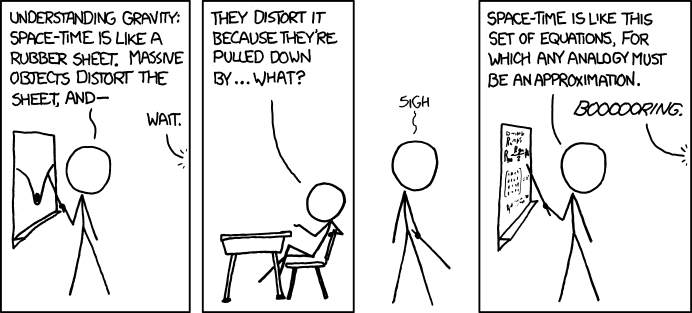
\includegraphics[width=\columnwidth, height=0.3\textheight]{res/xkcd/895_teaching_physics.png}
	}{\url{https://xkcd.com/895}}
\end{center}
\end{multicols}

\clearpage

\begin{multicols}{2}
\begin{center}
	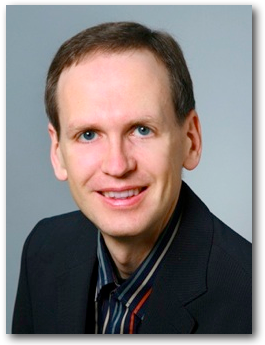
\includegraphics[width=\columnwidth, height=0.35\textheight]{res/vorstellungsfotos/alexander_kappes.png}\\
	Prof.\ Dr.\ Alexander Kappes\\
	Institut für Kernphysik
\end{center}

Mein Kollege Prof.\ Krüger und ich werden Sie in den nächsten 22~Monaten gemeinsam durch den "integrierten Kurs" (aka Physik~1--3) führen.
Für mich ist dies das erste Mal und dementsprechend gespannt bin ich auf dieses Abenteuer.
Das Physikstudium ist mit Sicherheit ein anspruchsvolles Studium.
Am Ende werden Sie aber mit einem tiefgreifenden Verständnis wichtiger Bereiche unserer komplexen Umwelt belohnt werden und sich ein Rüstzeug an Methoden und Wissen angeeignet haben, das Sie auch außerhalb der Physik in den verschiedensten Bereichen einsetzen werden können.

Ich selber habe Physik von 1992 bis 1997 an der Universität Bonn studiert und dort 2001 auf dem Gebiet der tief-inelastischen Elektron-Proton-Streuung am ZEUS-Experiment (DESY, Hamburg) promoviert.
Anschließend bin ich an die Universität Erlangen-Nürnberg gewechselt und forsche seitdem auf dem Gebiet der Hochenergie-Astroteilchenphysik mit Neutrinoteleskopen, zunächst mit dem ANTARES-Detektor, der auf dem Grund des Mittelmeers installiert ist.
Von 2006 bis 2008 verbrachte ich im Rahmen eines Marie-Curie-Forschungsstipendiums zwei Jahre an der Universität von Wisconsin-Madison, wo ich begann, am IceCube-Detektor zu arbeiten, einem \SI{1}{\km\cubed} großen Neutrinoteleskop am geographischen Südpol.
Nach meiner Rückkehr habe ich 2010 an der Universität Erlangen-Nürnberg auf dem Gebiet der Hochenergie-Neutrinoastronomie habilitiert.
Von 2010 bis 2013 hatte ich eine Vertretungsprofessur an der Humboldt-Universität zu Berlin inne, bevor ich dann zum Januar 2016 an die WWU berufen wurde.

An der WWU bin ich am Institut für Kernphysik tätig, wo ich mit meiner Gruppe auf dem Gebiet der Astroteilchen- und Neutrinophysik mit Neutrinoteleskopen forsche.
Hauptziel ist dabei ein besseres Verständnis des Hochenergieuniversums mit so gewaltigen Phänomenen wie supermassiven schwarze Löchern oder Supernova-Explosionen zu erlangen, in dem Atomkerne auf bis zu 10~Millionen mal höhere Energien beschleunigt werden, als dies mit irdischen Beschleunigern im Moment möglich ist.
Hierbei arbeiten wir zur Zeit hauptsächlich mit dem IceCube-Neutrinoteleskop, mit dem vor Kurzem erstmalig hochenergetische Neutrinos aus den Tiefen des Weltalls nachgewiesen werden konnten.
Wir sind an der Analyse der Daten des Detektors beteiligt und entwickeln einen verbesserten Sensor für den sich in der Planungsphase befindenden Nachfolgedetektor.
Die Astroteilchenphysik ist im Master-Studiengang Physik in der Vertiefungsrichtung "Kern- und Teilchenphysik" angesiedelt.

Ich freue mich auf unsere nächsten drei gemeinsamen Semester und hoffe, dass Physik Ihnen genauso viel Spaß machen wird wie mir.
Ich wünsche Ihnen einen erfolgreichen Start in das Physikstudium.
\end{multicols}

\begin{center}
	\fibelimgtext{
		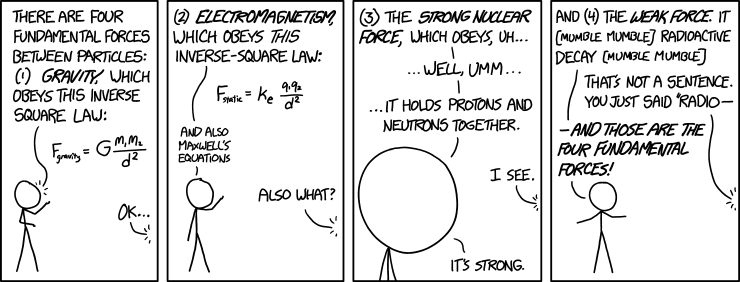
\includegraphics[width=0.9\textwidth, height=0.23\textheight]{res/xkcd/1489_fundamental_forces.png}
	}{\url{https://xkcd.com/1489}}
\end{center}

\clearpage

\begin{multicols}{2}
\begin{center}
	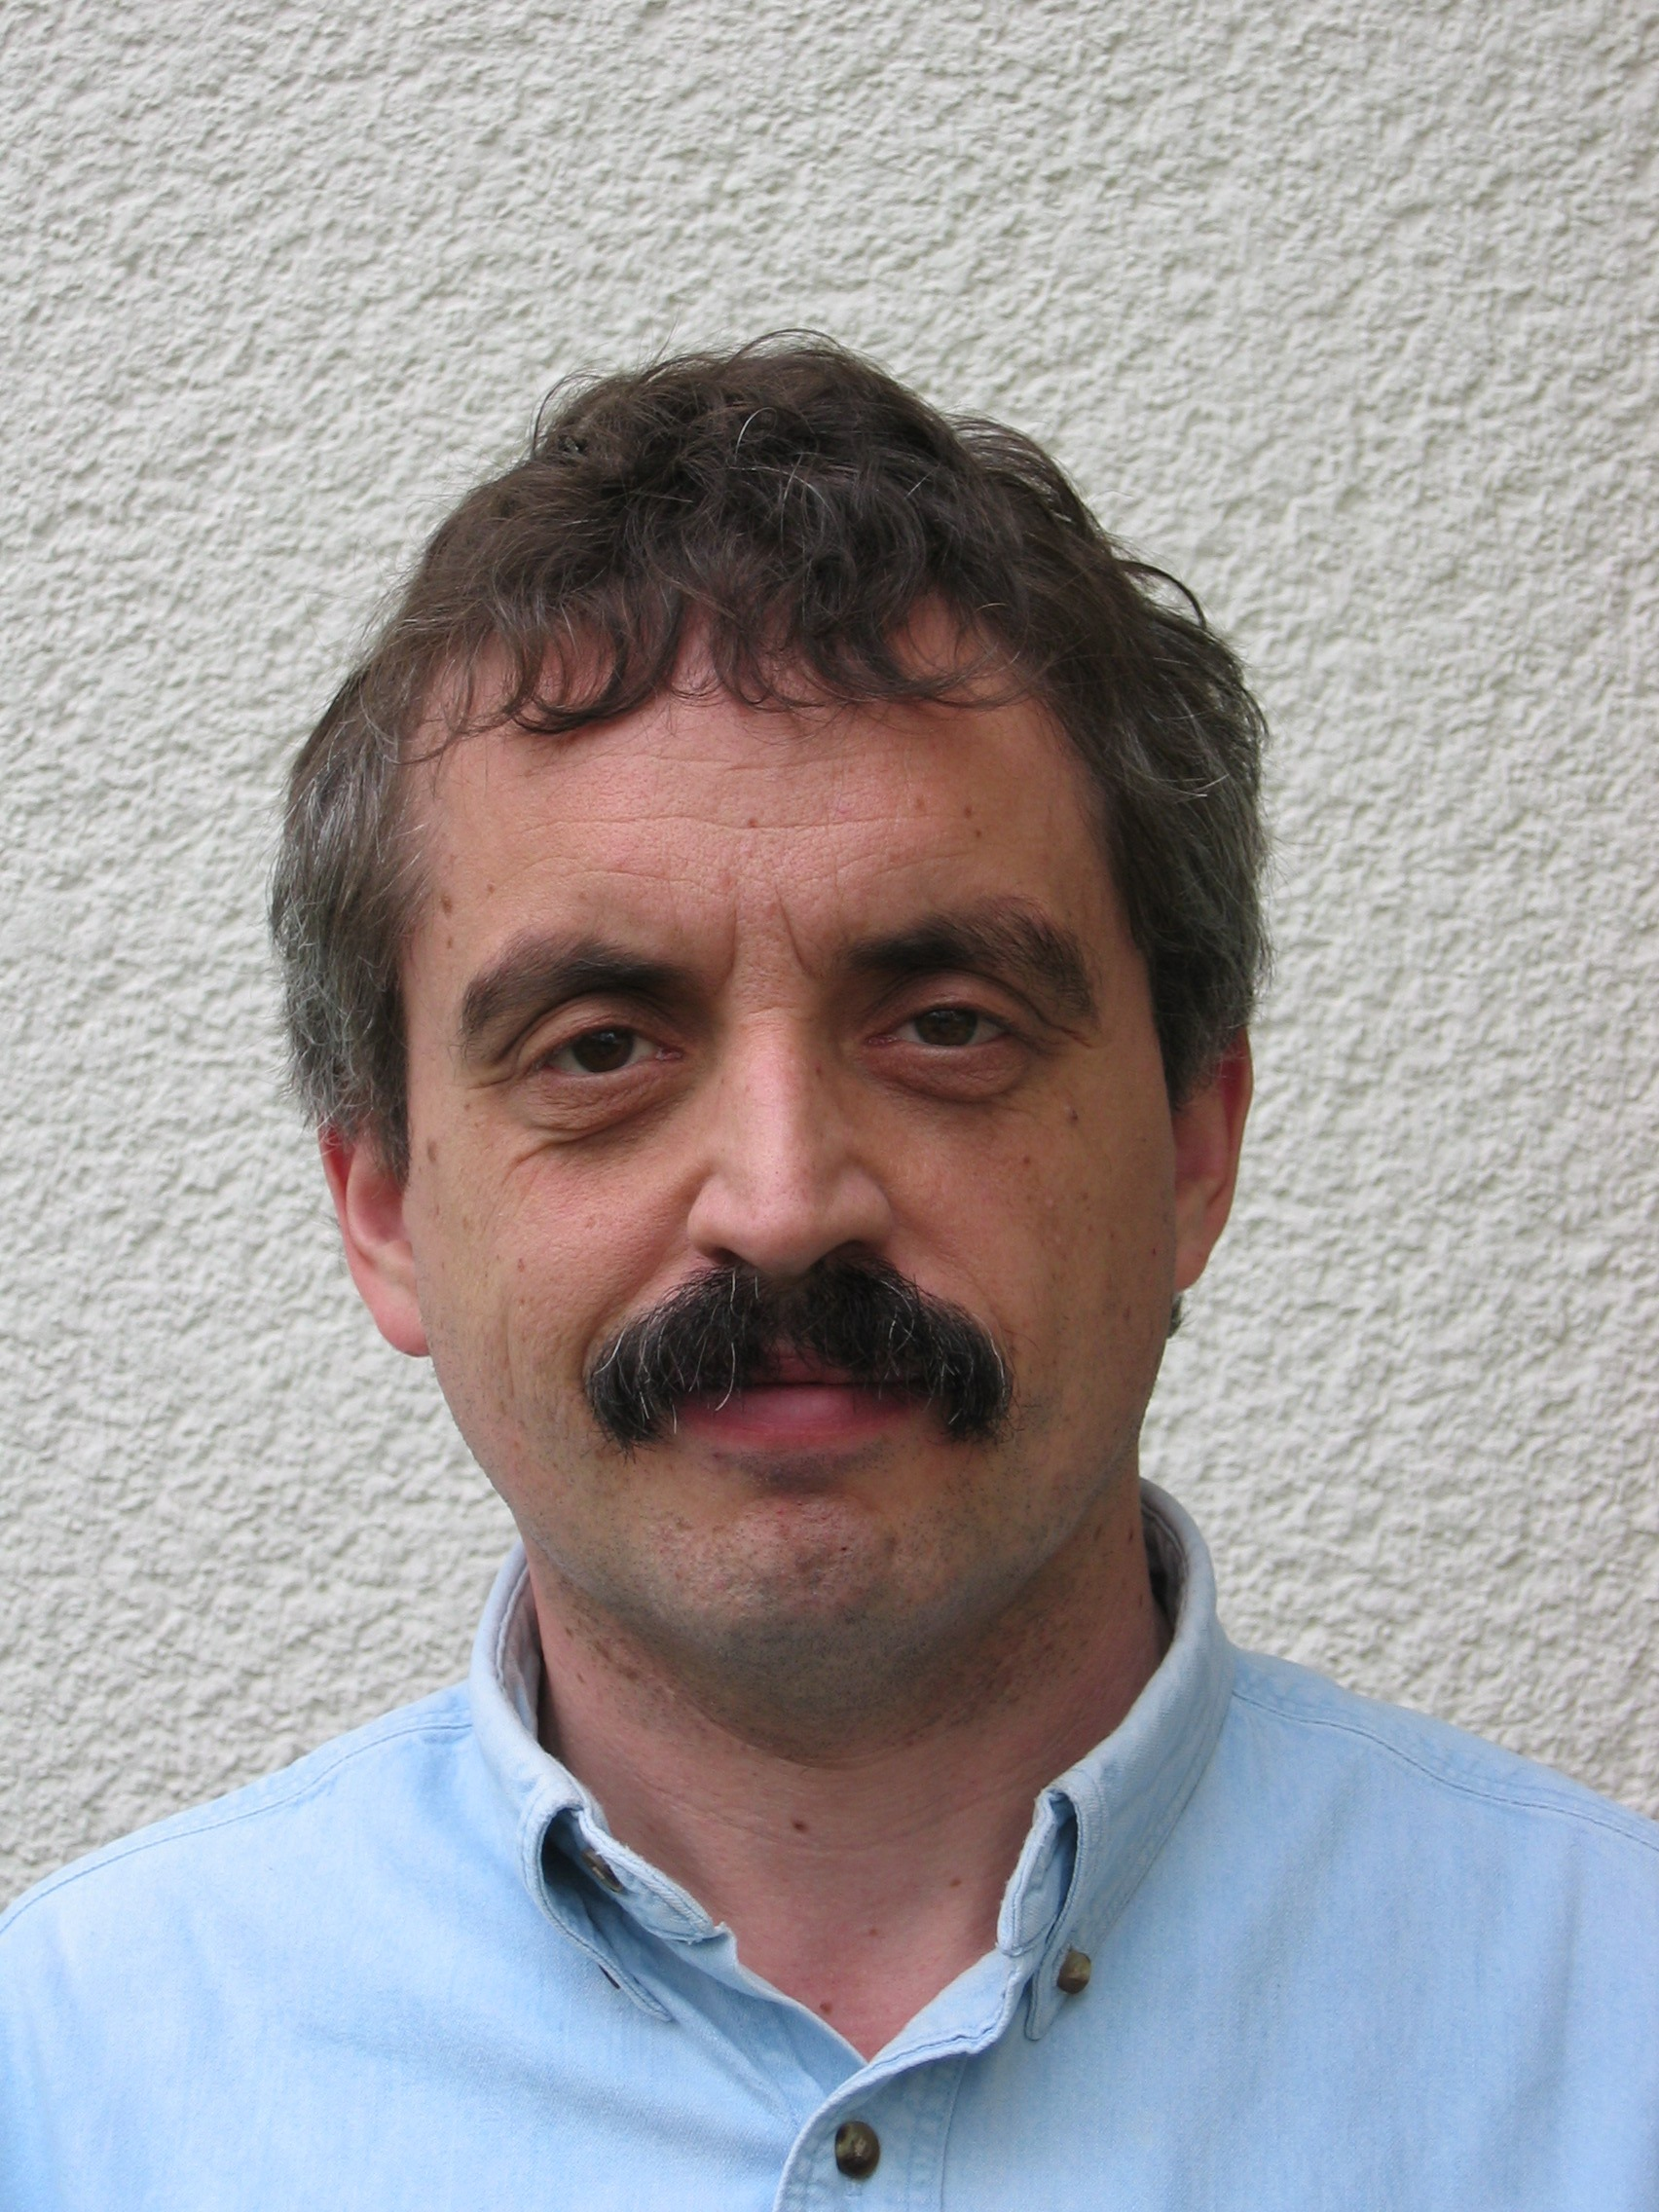
\includegraphics[width=\columnwidth, height=0.35\textheight]{res/vorstellungsfotos/wend_werner.jpg}\\
	Apl.\ Prof.\ Dr.\ Wend Werner\\
	Mathematisches Institut
\end{center}

Mir werden Sie in der nächsten Zeit in den Vorlesungen zur "Mathematik für Physiker" begegnen.
Mein Studium von Mathematik und Physik habe ich an der Freien Universität Berlin absolviert; Diplom und Promotion habe ich auch jeweils dort abgeschlossen.
Meine Habilitation habe ich an der Universität Paderborn gemacht und bin nun seit gut einem Jahrzehnt Hochschullehrer in Münster.

\[
	\resizebox{0.4\columnwidth}{!}{
		$\displaystyle\sum_{n = 1}^\infty \frac{1}{n^2} = \frac{\pi^2}{6}$
	}
\]

Die Themen von Promotion und Habilitation betrafen geometrische Fragen in Räumen unendlicher Dimension.
In letzter Zeit war das vor allem "Nichtkommutative Geometrie", ein Gebiet, welches versucht, einen mathematischen Formalismus zu finden, der in der Lage ist, Quanten- und relativistische Physik in einheitlicher Weise zu beschreiben.
Wie so oft beim Zusammenspiel von Mathematik und Physik sind auch hier interessante, rein mathematische Fragestellungen in Erscheinung getreten.

\begin{center}
	\includegraphics[width=\columnwidth, height=0.17\textheight]{private/res/comics/calvin_mathe.pdf}
\end{center}

Der Zyklus "Mathematik für Physiker" ist eine kleine Herausforderung, da in vergleichsweise kurzer Zeit eine größere Stoffmenge vermittelt werden muss, die nichtsdestotrotz von den Teilnehmern anschließend handwerklich beherrscht werden muss.

Aber, keine Angst: Wir werden sehr langsam beginnen und erst im Laufe der Zeit Fahrt aufnehmen.

\begin{center}
	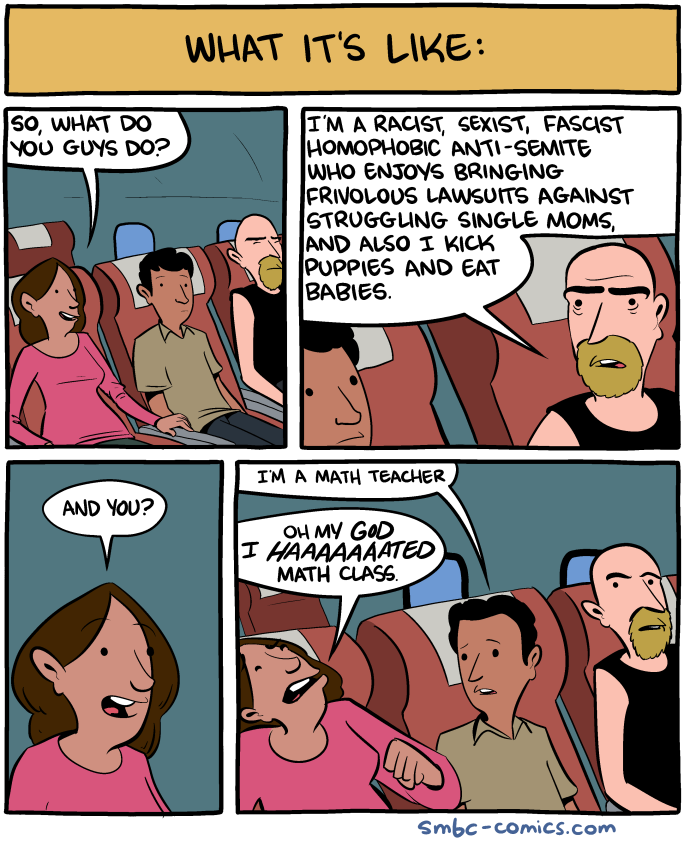
\includegraphics[width=\columnwidth, height=0.32\textheight]{res/smbc/2016-06-19_what-its-like.png}
\end{center}
\end{multicols}

\begin{center}
	\fibelimgtext{
		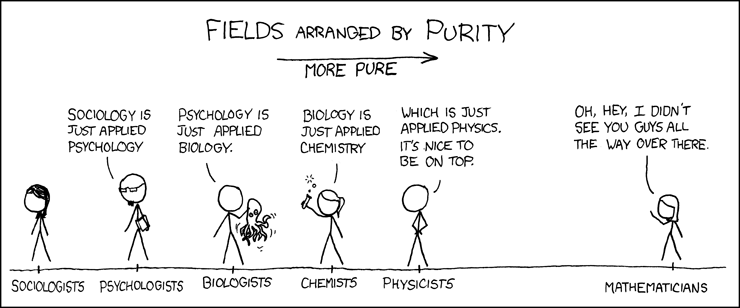
\includegraphics[width=0.9\textwidth, height=0.22\textheight]{res/xkcd/435_purity.png}
	}{\url{https://xkcd.com/435}}
\end{center}
